\label{chp:results}

After introducing the implementation of the \emph{ab initio} Green Kubo (aiGK) method in the previous chapter, we are now in position to present results for the set of potential thermal insulators identified in chapter~\ref{chp:anharmonicity}.

We first discuss the question of simulation time convergence for an initial set of materials in order to predict systems which can be computed with a simulation time of 30-60\,ps. This time was chosen as a compromise between the finite amount of available computational ressources, and the desire to compute as many materials from the list of candidates as possible.
% 57 materials
%
In a second step, we compare the computed thermal conductivities at room temperature to experimental references for the subset of materials where experiments are available to further verify the aiGK method beyond the two materials presented in the previous chapter.
% 22 materials 
%
In the last step, we present the computed thermal conductivities for the remaining materials,~i.\,e.,~those where no experimental thermal conductivity was reported before, and discuss how they fit into the schema of predicting thermal insulators from anharmonicity estimation as discussed in Sec.\,\ref{sec:kappa_vs_sigmaA}.
\idea{we highlight some materials with noteworthy properties and try to answer some open question in the experimental literature}

\idea{compare to theoretical approaches, i.e., the Roekeghem perovskites}



\section{Convergence estimation}

\begin{figure}
	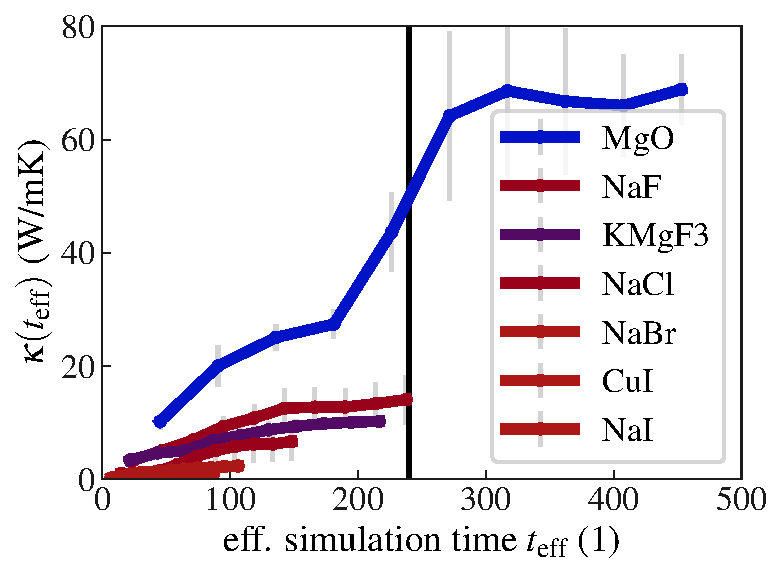
\includegraphics[width=.49\textwidth]{./data/plots/kappa_convergence/3.pdf}
	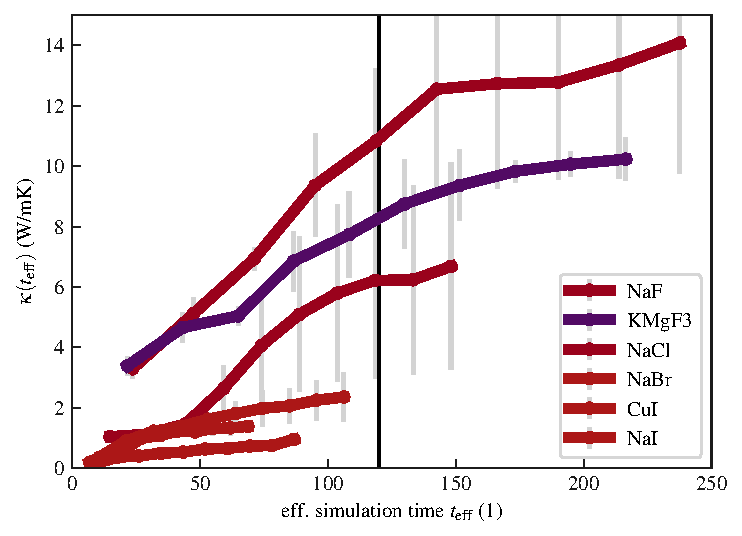
\includegraphics[width=.49\textwidth]{./data/plots/kappa_convergence/4.pdf}
	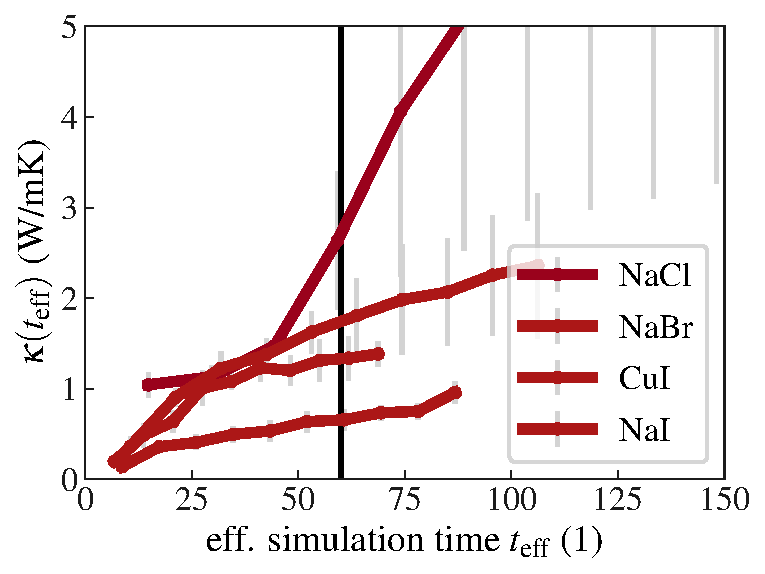
\includegraphics[width=.49\textwidth]{./data/plots/kappa_convergence/5.pdf}
	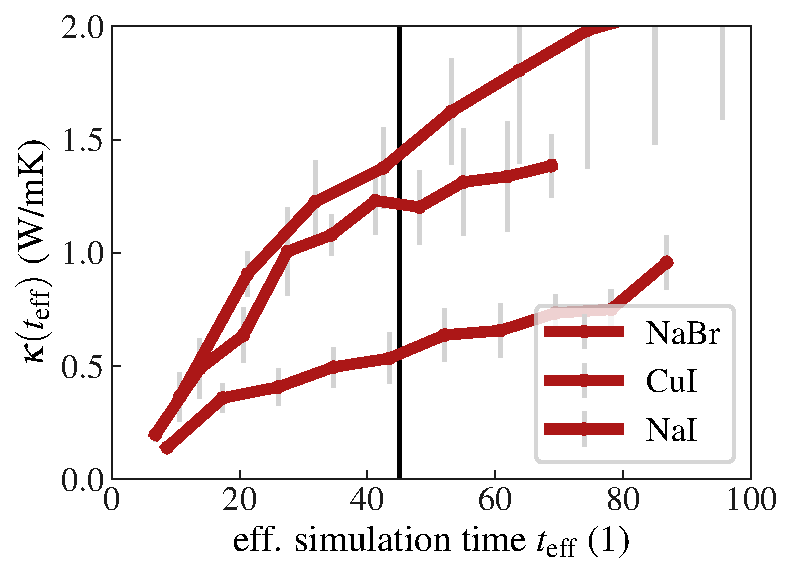
\includegraphics[width=.49\textwidth]{./data/plots/kappa_convergence/6.pdf}
	\caption{Illustration of minimal necessary effective simulation times. Upper left: $\teff = 240$ for harmonic materials with $\sigmaA \leq 0.2$. Upper right: $\teff = 120$ for materials with $0.2 < \sigmaA \leq 0.3$. Lower left: $\teff = 60$ for materials with $0.3 < \sigmaA \leq 0.4$. Lower right: $\teff = 45$ for materials with $\sigmaA > 0.4$.}
	\label{fig:kappa_convergence_trustlevel}
\end{figure}


\section{Comparision to Experiment}

\begin{figure}
	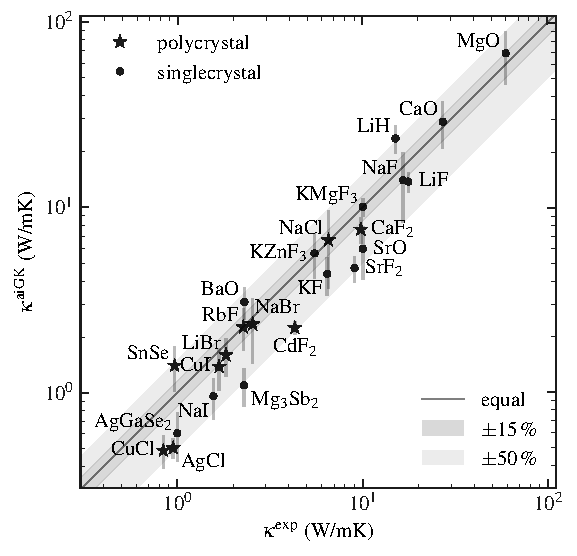
\includegraphics[width=\textwidth]{./data/plots/kappa_vs_exp_trusted/kappa_vs_exp_corrected_annotated.pdf}
	\caption{Comparison to experiment. Bullets($\bullet$): Single crystal. Stars ($\star$): Contains data from polycrystalline experiment. Error bar in y-direction: Statistical uncertainty for $\kappa^{\rm aiGK}$ from standard error over individual trajectories. Diagonal line: Agreement with experiment or mean of experiments if multiple available. Dark grey region: Agreement between mean experiment and mean computation with $\pm 15\,\%$ deviation. Light grey region: Agreement between mean experiment and mean computation with $\pm 50\,\%$ deviation.}
	\label{fig:kappa_exp}
\end{figure}



\section{Relation to Anharmonicity}

\begin{figure}
	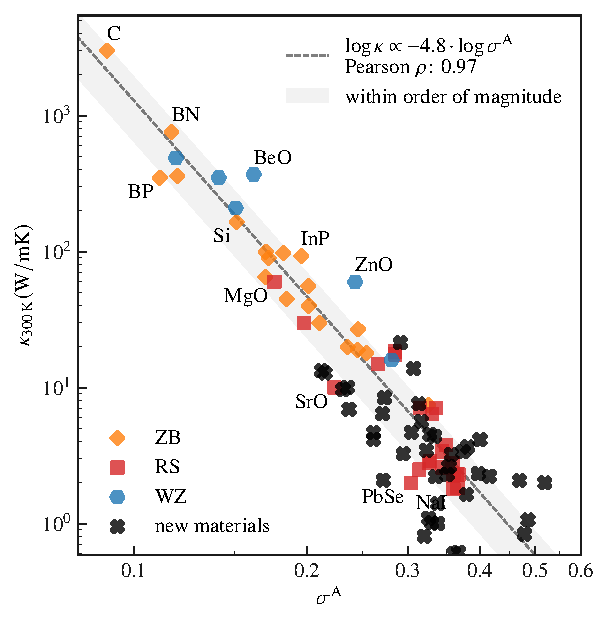
\includegraphics[width=\textwidth]{./data/plots/anharmonicity/9_kappa/incl_computations/sigma_vs_kappa_annot_comp.pdf}
	\caption{Thermal conductivity at room temperature vs. anharmonicity measure.}
	\label{fig:kappa_sigma_exp_comp}
\end{figure}

\begin{figure}
	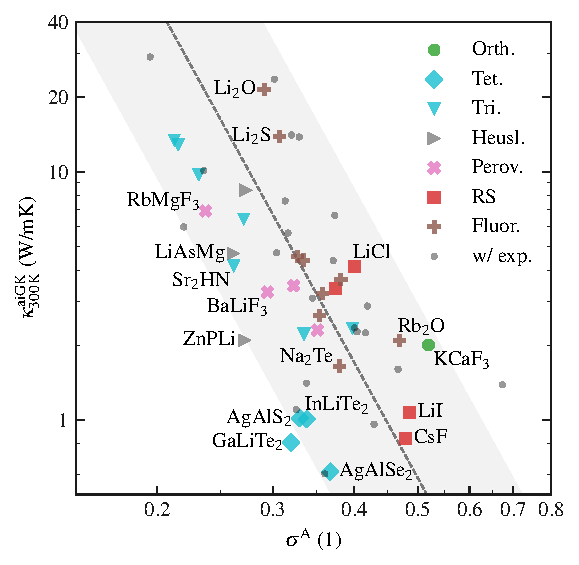
\includegraphics[width=\textwidth]{./data/plots/kappa_vs_sigma_trusted/kappa_vs_sigma_trusted.pdf}
	\caption{Thermal conductivity at room temperature vs. anharmonicity measure. Small grey dots denote materials where experimental reference was available. Other symbols denote materials where not experimental references where available before.}
	\label{fig:kappa_sigma}
\end{figure}

\newpage

\subsection{Chalcopyrites}
\begin{figure}
	\centering
	GaLiTe$_2$ \hspace{3.7cm} InLiTe$_2$\\
	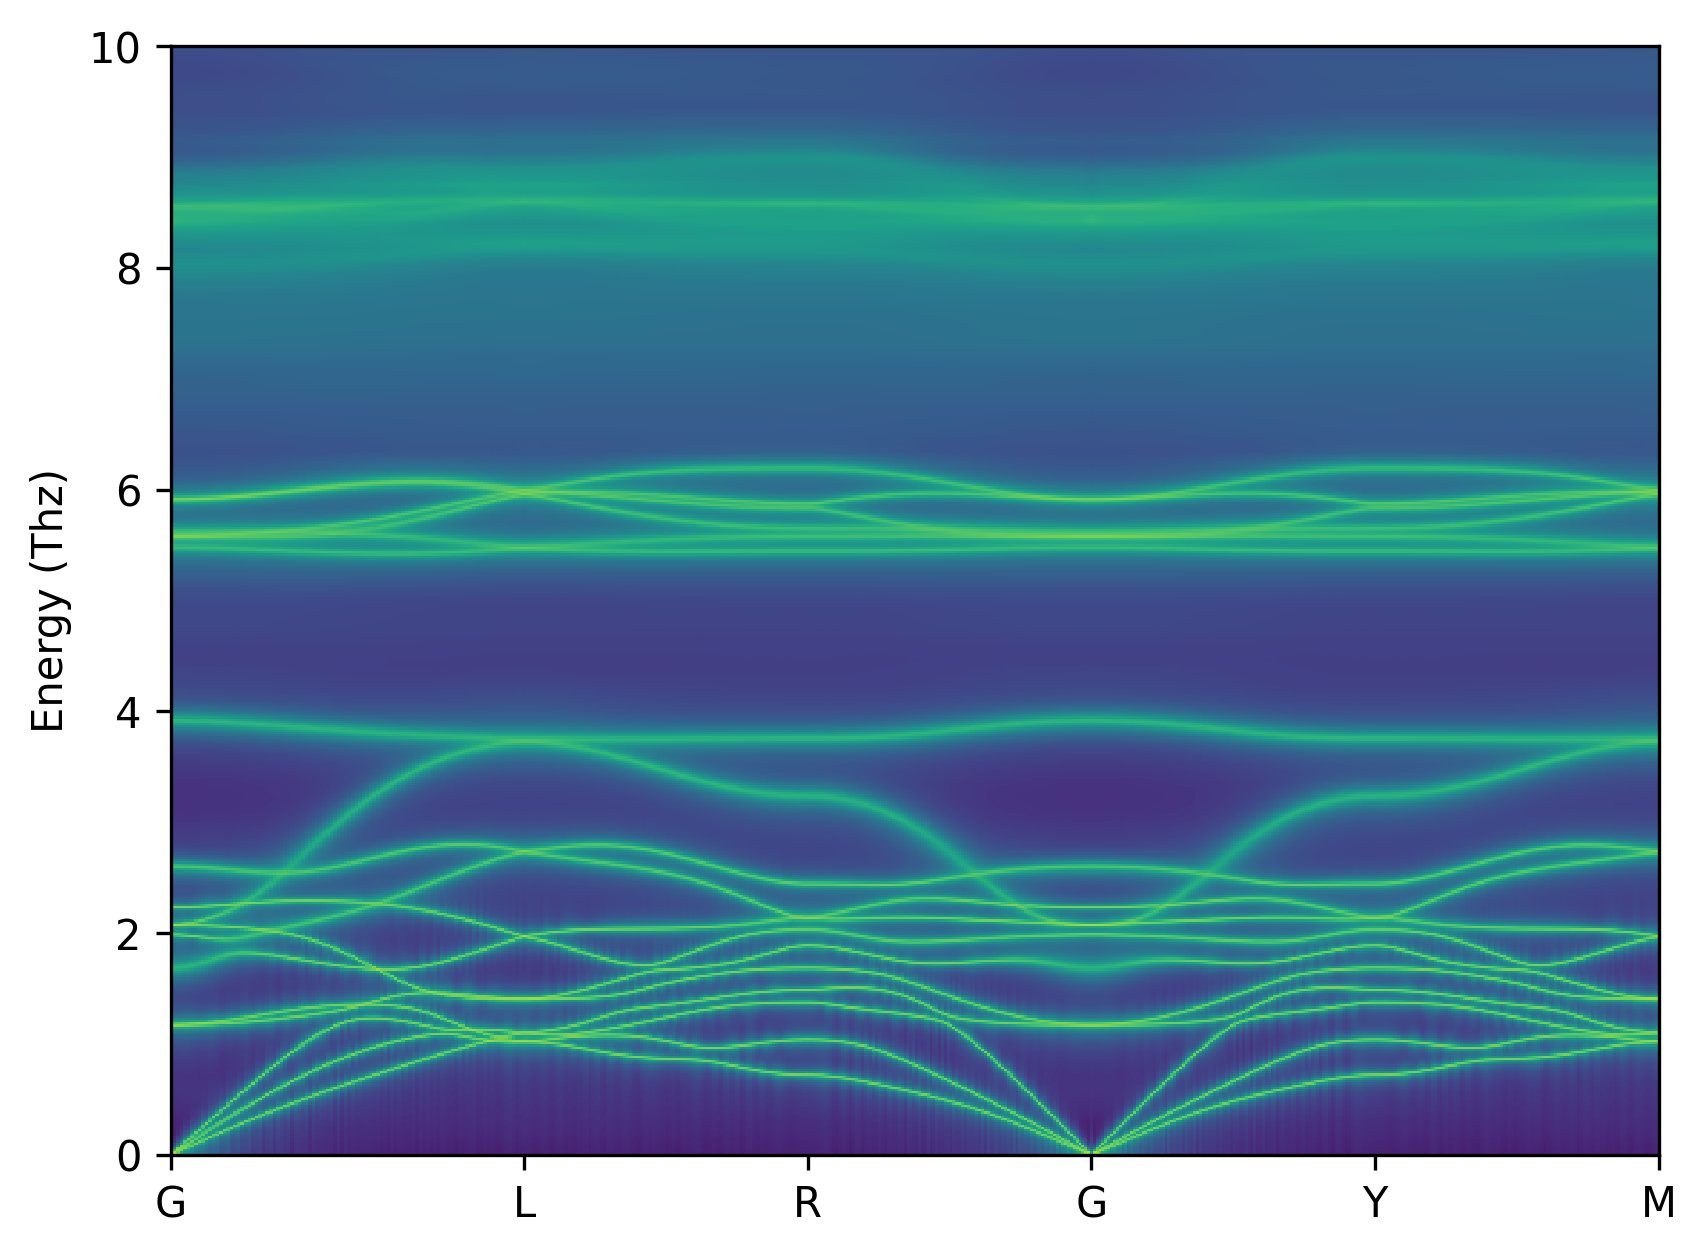
\includegraphics[width=0.45\textwidth]{./data/plots/spectral_functions/122.04.GaLiTe2.png}
	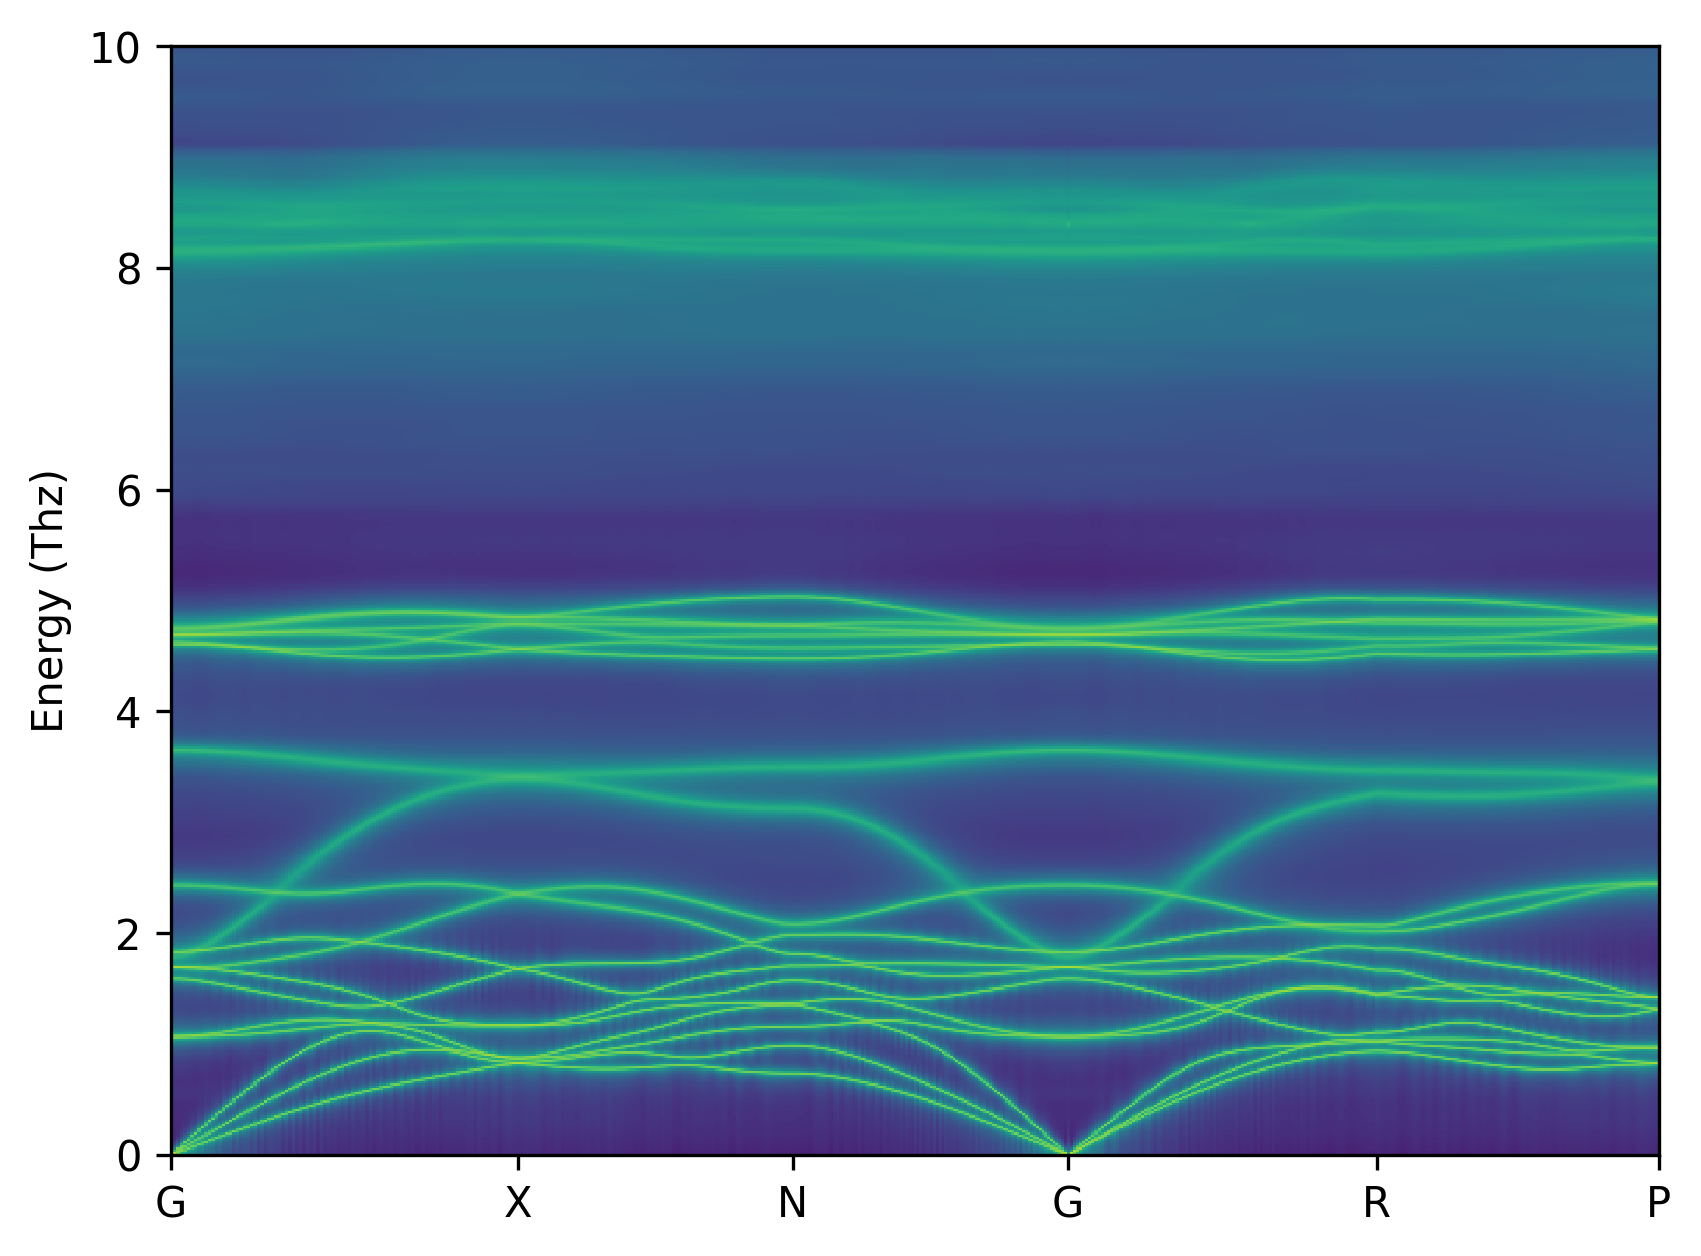
\includegraphics[width=0.45\textwidth]{./data/plots/spectral_functions/122.04.InLiTe2.png}
	\caption{Spectral functions for the chalcopyrite materials GaLiTe$_2$ and InLiTe$_2$.}
	\label{fig:kappa_sigma}
\end{figure}

\cite{kuhn1985,kuhn1987,isaenko2005}

\begin{table}[ht]
  \centering
  \fontfamily{ppl}\selectfont
\begin{tabular}{lrrr}
\toprule
     material &  kappa\_corrected &      sigma &  space\_group \\
\midrule
 InLiTe$_2$ &             0.46 &       0.33 &          122 \\
 GaLiTe$_2$ &             0.47 &       0.31 &          122 \\
  AgAlS$_2$ &             0.84 &       0.33 &          122 \\
        CsF &             0.84 &       0.48 &          225 \\
        LiI &             1.07 &       0.49 &          225 \\
   Na$_2$Te &             1.64 &       0.38 &          225 \\
   KCdF$_3$ &             1.67 &       1.32 &           62 \\
   KCaF$_3$ &             2.00 &       0.52 &           62 \\
    Rb$_2$O &             2.08 &       0.47 &          225 \\
      ZnPLi &             2.09 &       0.27 &          216 \\
 InNaSe$_2$ &             2.22 &       0.34 &          166 \\
  CsCdF$_3$ &             2.30 &       0.35 &          221 \\
 InLiSe$_2$ &             2.34 &       0.40 &          166 \\
   Na$_2$Se &             2.63 &       0.35 &          225 \\
   Li$_2$Te &             3.24 &       0.36 &          225 \\
  BaLiF$_3$ &             3.27 &       0.29 &          221 \\
         KH &             3.39 &       0.37 &          225 \\
  RbZnF$_3$ &             3.47 &       0.32 &          221 \\
     K$_2$O &             3.67 &       0.38 &          225 \\
       LiCl &             4.14 &       0.40 &          225 \\
   Sr$_2$HN &             4.17 &       0.26 &          166 \\
    Na$_2$S &             4.40 &       0.33 &          225 \\
   Li$_2$Se &             4.55 &       0.33 &          225 \\
     LiAsMg &             4.67 &       0.26 &          216 \\
  LiScS$_2$ &             6.42 &       0.27 &          166 \\
  RbMgF$_3$ &             6.94 &       0.24 &          221 \\
      LiNZn &             8.42 &       0.27 &          216 \\
  InNaO$_2$ &             9.71 &       0.23 &          166 \\
  CuGaO$_2$ &            12.82 &       0.22 &          166 \\
  LiRhO$_2$ &            13.37 &       0.21 &          166 \\
    Li$_2$S &            13.85 &       0.31 &          225 \\
    Li$_2$O &            21.39 &       0.29 &          225 \\
\bottomrule
\end{tabular}
  \caption{Thermal conductivities without experimental reference.}
  \label{tab:kappa.noexp}
\end{table}